\documentclass{article}
\usepackage{amsmath}
\usepackage{amsfonts}
\usepackage{amssymb}
\usepackage{multicol}
\usepackage{graphicx}

\graphicspath{ {./images/} }

\setlength{\parindent}{0pt}

\begin{document}

\section*{Problem Set 1}

1. Find the area of region bounded by the x-axis, $x=-2$, $x=3$, and $y=|x+1|$.
\\\\
\textbf{Solution:}

\begin{align*}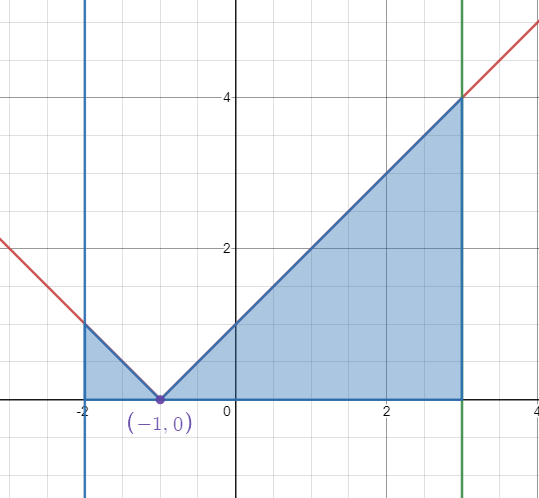
\includegraphics[scale=0.45]{problemset1_1.PNG}\end{align*}
\begin{align*}
    A &= \int_{-2}^{-1} -(x+1) \, dx + \int_{-1}^{3} \, x+1 \, dx \\
    &= -\int_{-2}^{-1} x+1 \, dx + \int_{-1}^{3} \, x+1 \, dx \\
    &= \left[\frac{x^2}{2} + x\right]_{-2}^{-1} + \left[\frac{x^2}{2} + x\right]_{-1}^{3} \\
    &= \left(\frac{1}{2}\right) + \left(\frac{15}{2} + \frac{1}{2}\right) \\
    &= \frac{17}{2}
\end{align*}

2. If $\frac{df}{dx} = e^x-2x$ and $f(0) = 2$, obtain $f(x)$.
\\\\
\textbf{Solution:}

\begin{align*}
    \int \frac{df}{dx} \,dx  &= f(x) + C  \\
    \int e^x-2x \,dx  &= f(x) + C \\
    e^x-x^2  &= f(x) + C \\
\end{align*}

\,\,\,\, If f(0) = 2, then:
\begin{align*}
    e^0-x^0  &= 2 + C \\
    1 + C  &= 2 \\
    C &= 1
\end{align*}

\,\,\,\, Thus: \[f(x) = e^x-x^2+1\]

5. Write the following limit of a Riemann sum as a definite integral and obtain its value:
\[\lim_{n \rightarrow \infty} \frac{1^2+2^2+\text{...}+n^2}{n^3}\]
\\
\textbf{Solution:}\\
Rewrite:

\end{document}